\documentclass{article}
\usepackage[margin=1in]{geometry}
\usepackage[utf8]{inputenc}
\usepackage[english]{babel}
\usepackage{amssymb}
\usepackage{amsmath}
\usepackage{gensymb}
\usepackage{graphicx}
\usepackage{ragged2e}
\usepackage{blindtext}
\usepackage{setspace}
\usepackage{tabularx}
\setlength{\parindent}{4em}
\setlength{\parskip}{1em}
\renewcommand{\baselinestretch}{1.0}

\begin{titlepage}
\clearpage\thispagestyle{empty}
\title{%
   \large{Univerzita Karlova}\\
    \vspace{1cm}\\
   \large{Přírodovědecká fakulta}\\
\vspace{2cm}\\
\[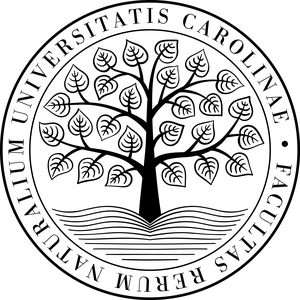
\includegraphics[height=60mm]{images/logo_uk.PNG}\]
\vspace{2cm}\\
   \Large{Úloha 4 - Množinové operace s polygony}\\
   \vspace{1cm}\\
  \large{Algoritmy počítačové kartografie}
\vspace{3cm}\\
    \large{Tomáš Hřebec, Kateřina Obrazová}\\
    \date{Praha 2022}}
\end{titlepage}
\begin{document}
\maketitle
\thispagestyle{empty}
\doublespacing
\section{\large{Zadání úlohy}}
\subsection{\small{Povinná část}}
\justifying
\emph{Vstup: Nekonvexní polygony $P, Q,$}\\
\emph{Výstup: množina k polygonů $P'$ = \{$P_{1}', ..., P'_{k}$\}.}\\
S využitím algoritmu pro množinové operace s polygony implementujte pro dvojici polygonů $P, Q$ následující množinové operace:\begin{itemize}
    \item průnik polygonů, 
    \item sjednocení polygonů,
    \item rozdíl polygonů.
\end{itemize}
Jako vstupní data použijte existující kartografická či syntetická data reprezentující množiny $P, Q$, která budou načítána ze dvou textových souborů ve Vámi zvoleném formátu.\\
Grafické rozhraní realizujte s využitím frameworku QT, výsledky množinových operací vizualizujte.\\
Poznámka: pro výše uvedené kroky je nutné mít řádně odladěny algoritmy z úlohy 1.\\
\subsection{\small{Volitelná část}}
V této úloze nebyly řešené bonusové úlohy.
\clearpage
\newpage
\section{\large{Formulace problému}}
Na vstupu je dvojce množin. Tyto množiny jsou uzavřené a ohraničené polygony (oblasti) $A$ a $B$. (Obr. 1) Hledáme základní množinové operace mezi nimi - průnik, sjednocení a rozdíl.
\[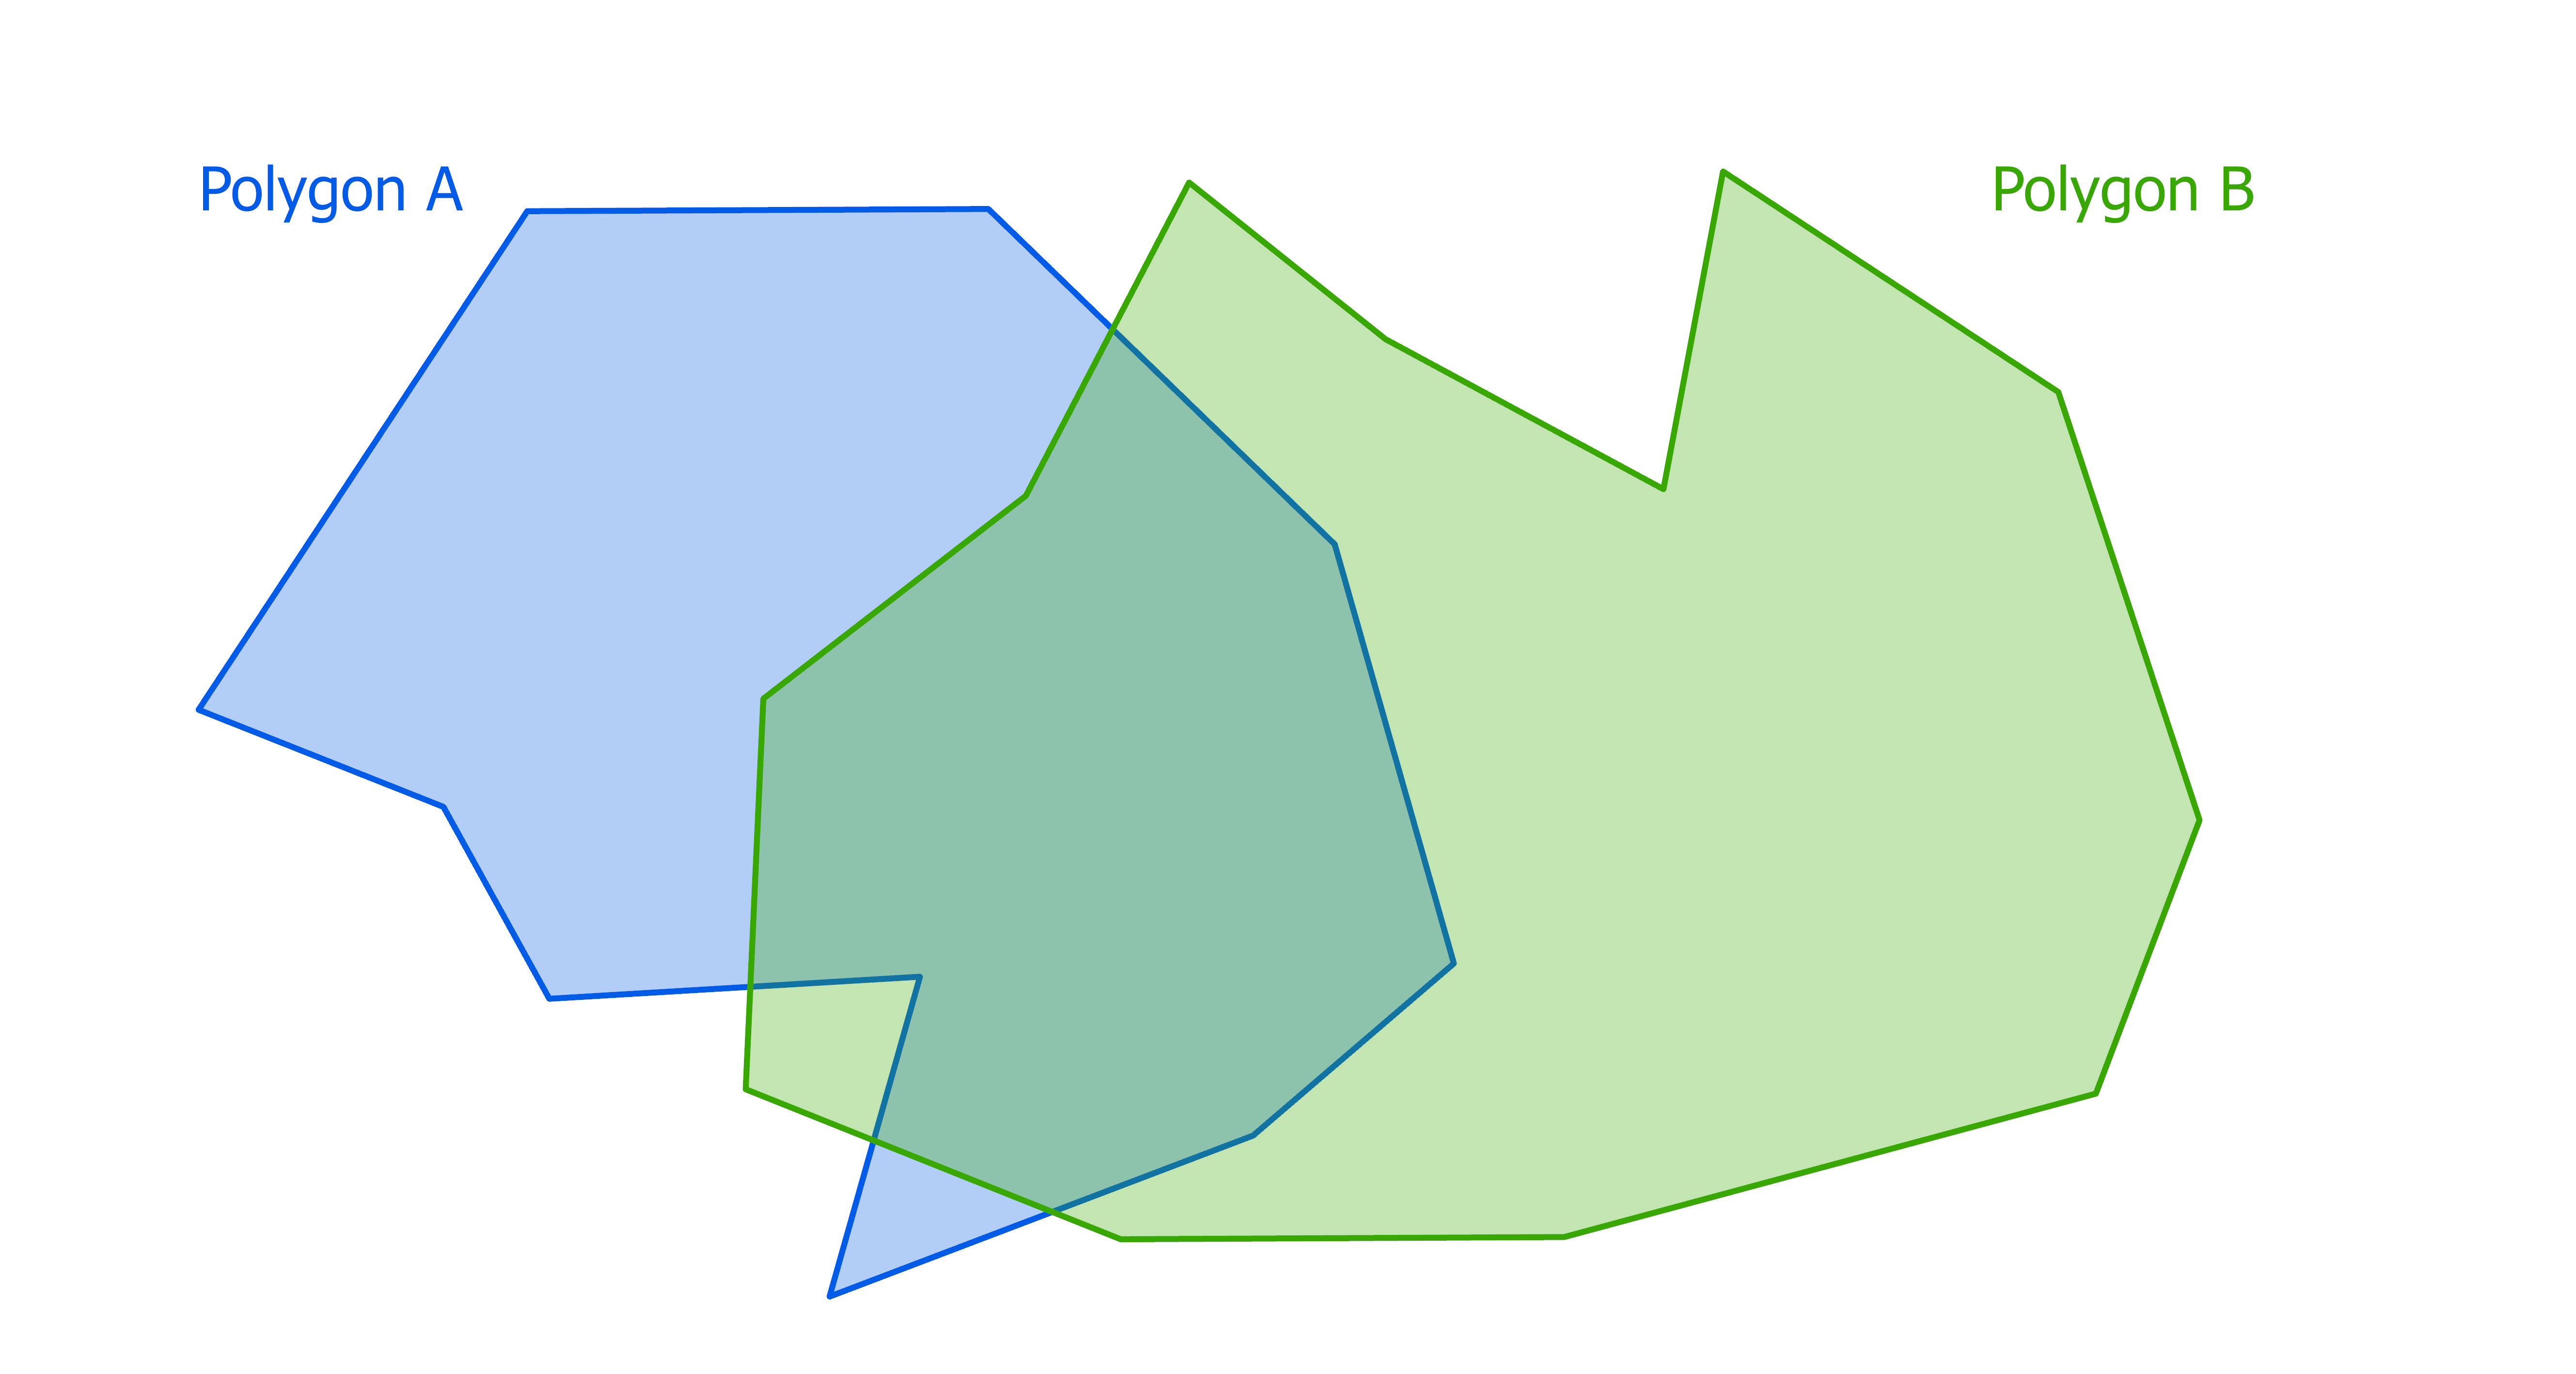
\includegraphics[height=35mm]{images/polygony.PNG}\]
\[\textit{\footnotesize{Obr. 1 - Příklad polygonů A a B}}\]
Průnik množin $A$ a $B$ (angl. \emph{Intersetion}) je množinou všech prvků obsažených v množině $A$, a zároveň i v množině $B$. (Obr. 2) Značí se jako $A \cap B$. (Moravec 2008)\\
\[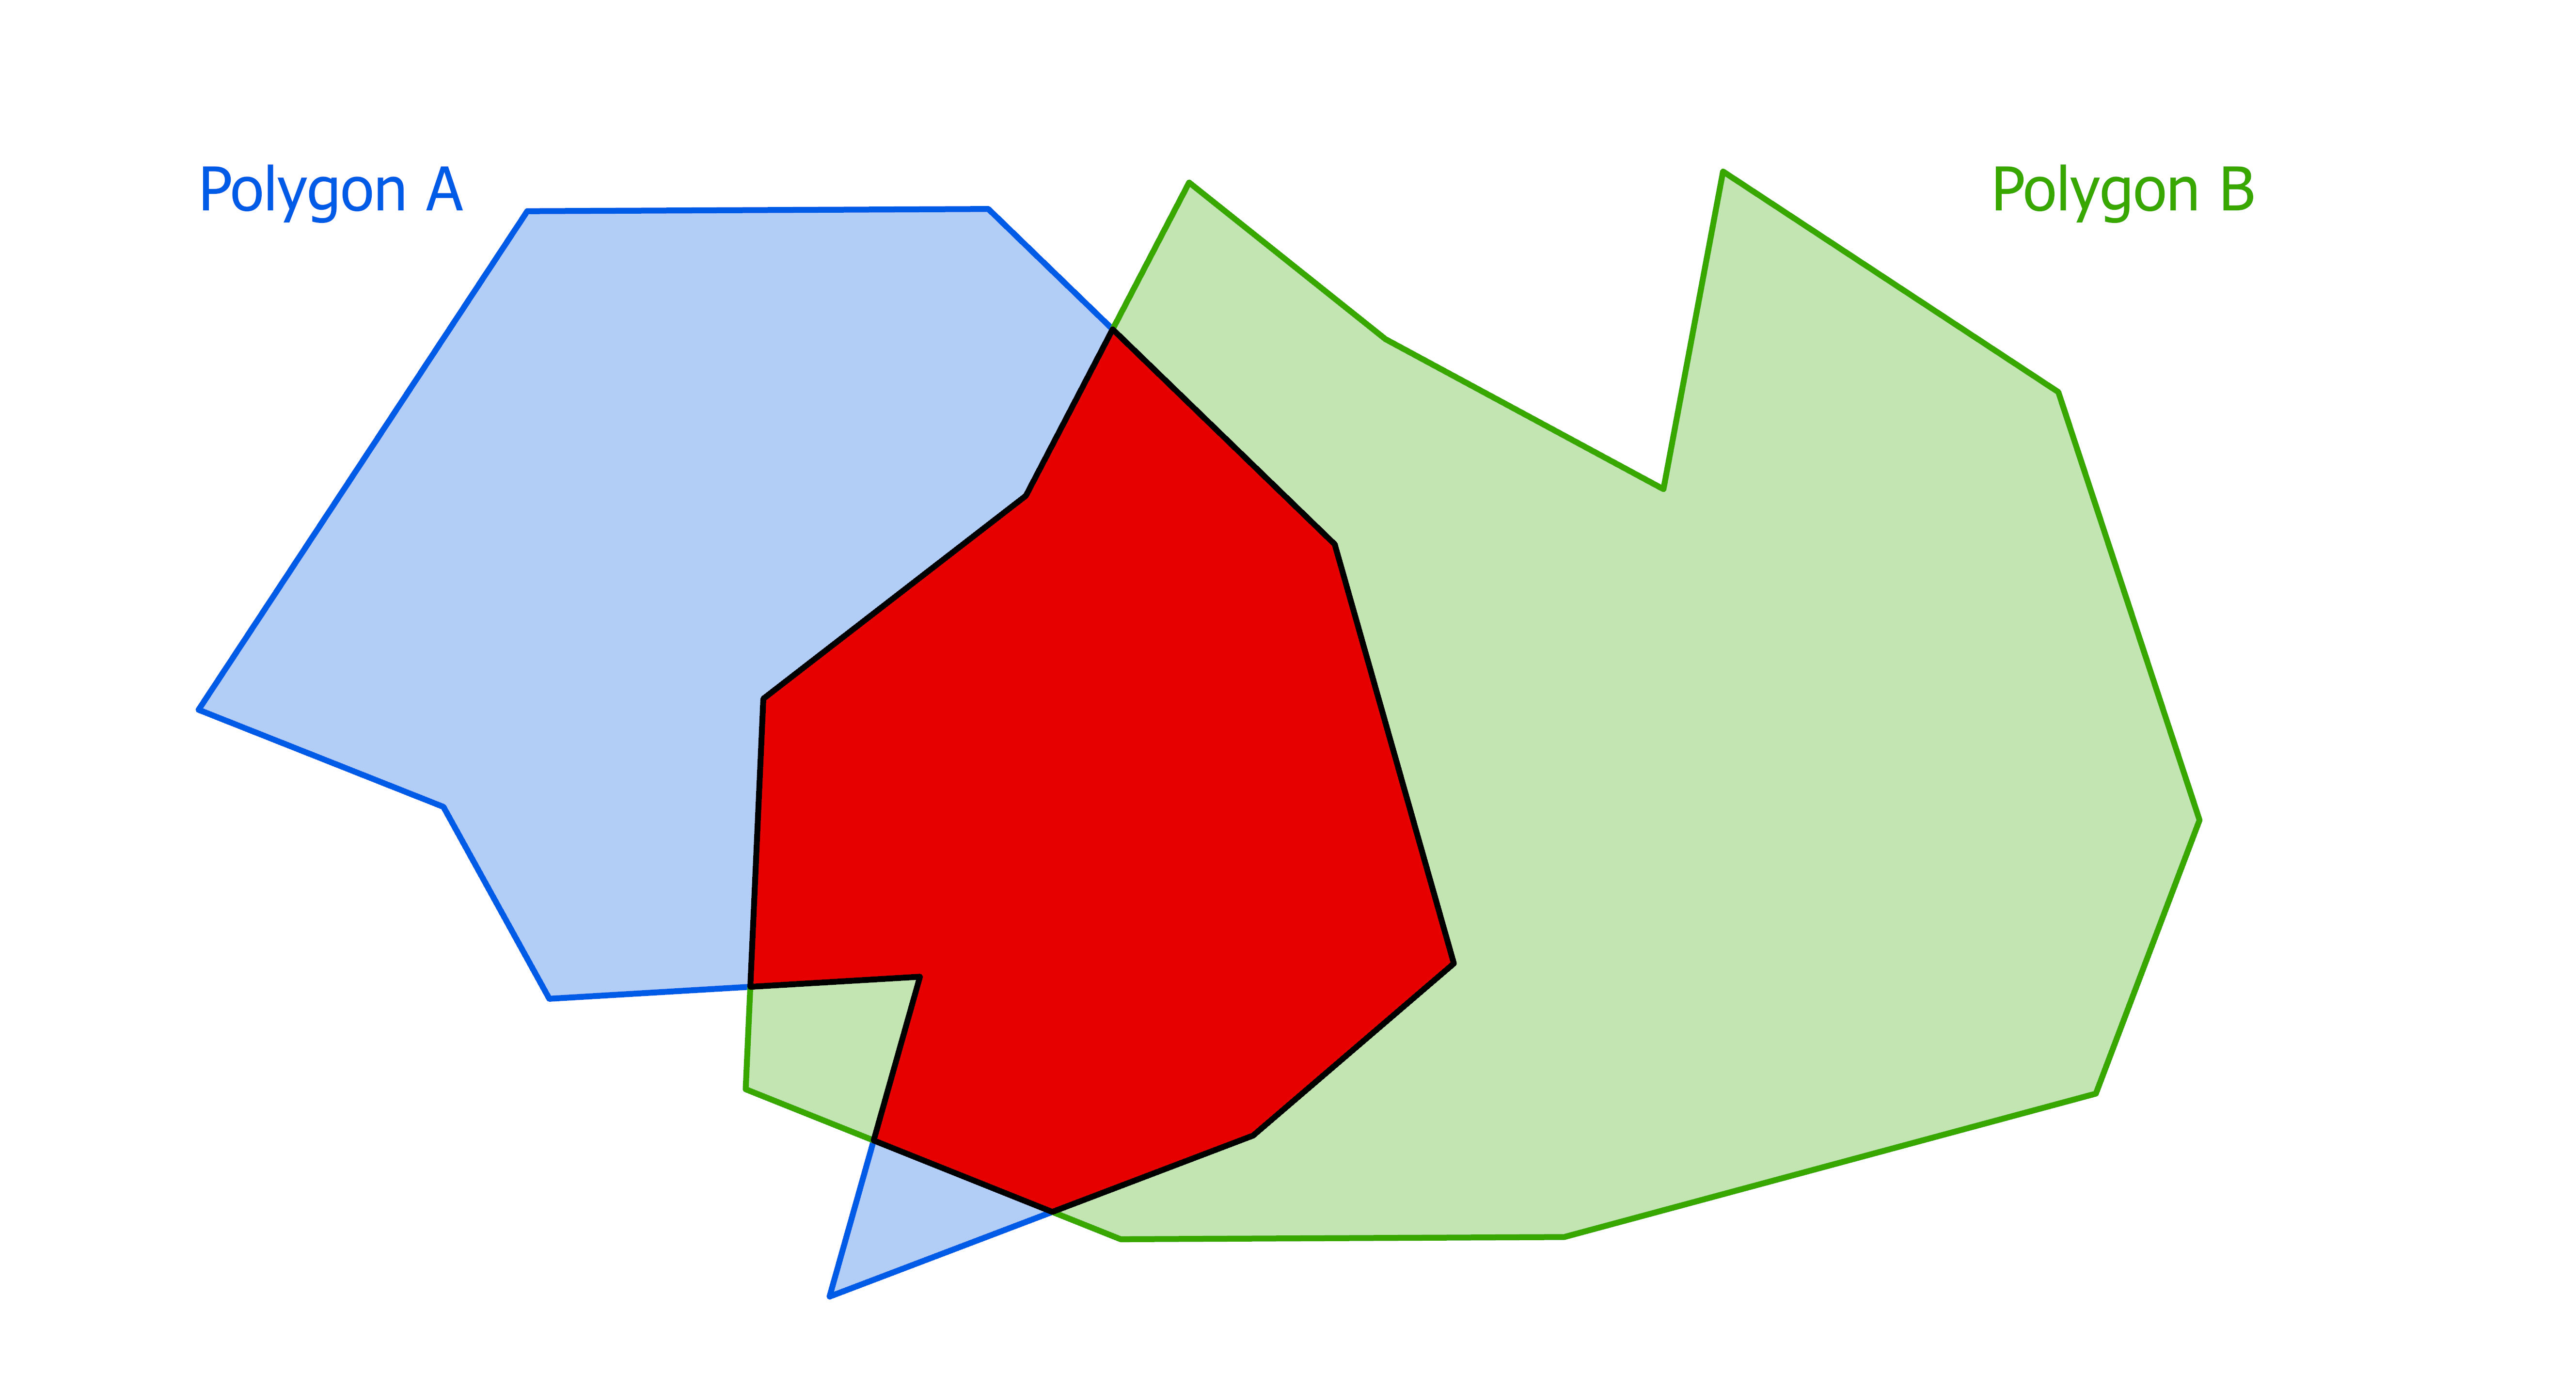
\includegraphics[height=35mm]{images/intersect.PNG}\]
\[\textit{\footnotesize{Obr. 2 - Průnik polygonů A a B}}\]
Sjednocení množin $A$ a $B$ (angl. \emph{Union}) obsahuje jen a pouze takové prvky, které patří alespoň do jedné z množin $A$ a $B$. (Obr. 3) Značí se jako $A \cup B$. (Moravec 2008)\\
\[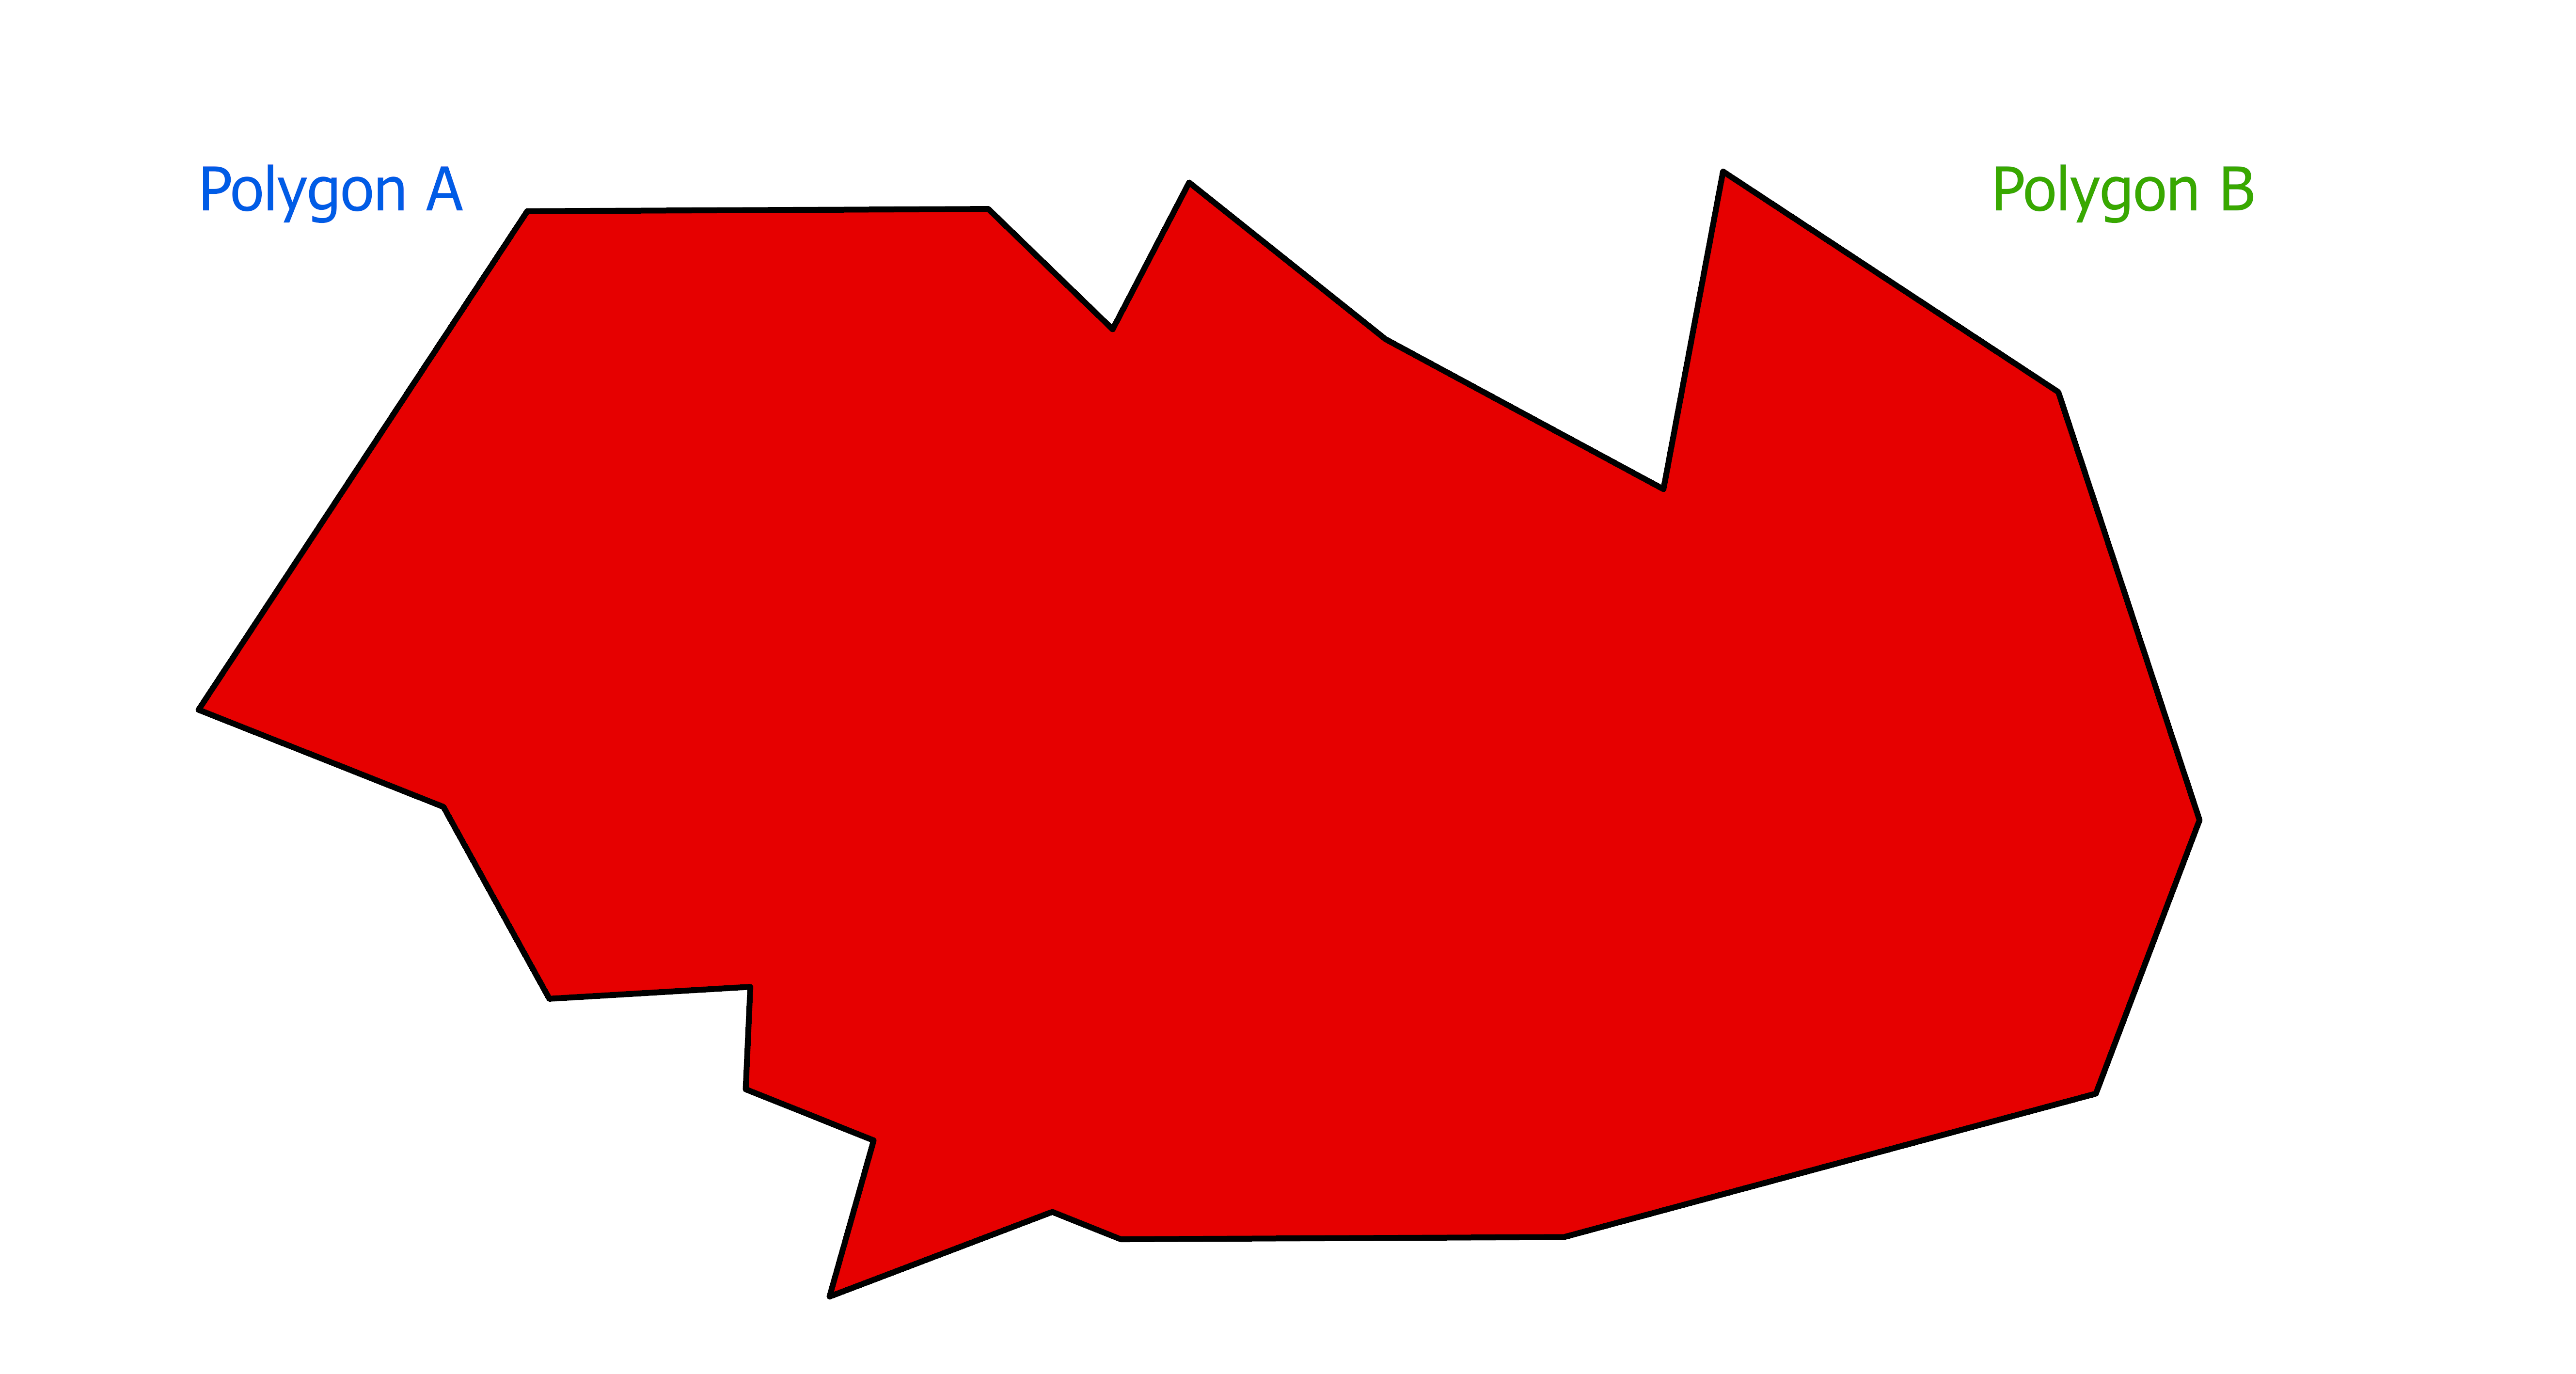
\includegraphics[height=35mm]{images/union.PNG}\]
\[\textit{\footnotesize{Obr. 3 - Sjednocení polygonů A a B}}\]
Rozdíl množin $A$ a $B$, respektive $B$ a $A$  (angl. \emph{Difference}), je množinou obsahující všechny prvky množiny $A$ (resp. $B$) s výjimkou těch, které jsou zároveň prvky množiny $B$ (resp. $A$). Značí se jako $A \cap \overline{B}$ (Obr. 4), respektive $\overline{A} \cap B$(Obr. 5). (Moravec 2008)\\
\[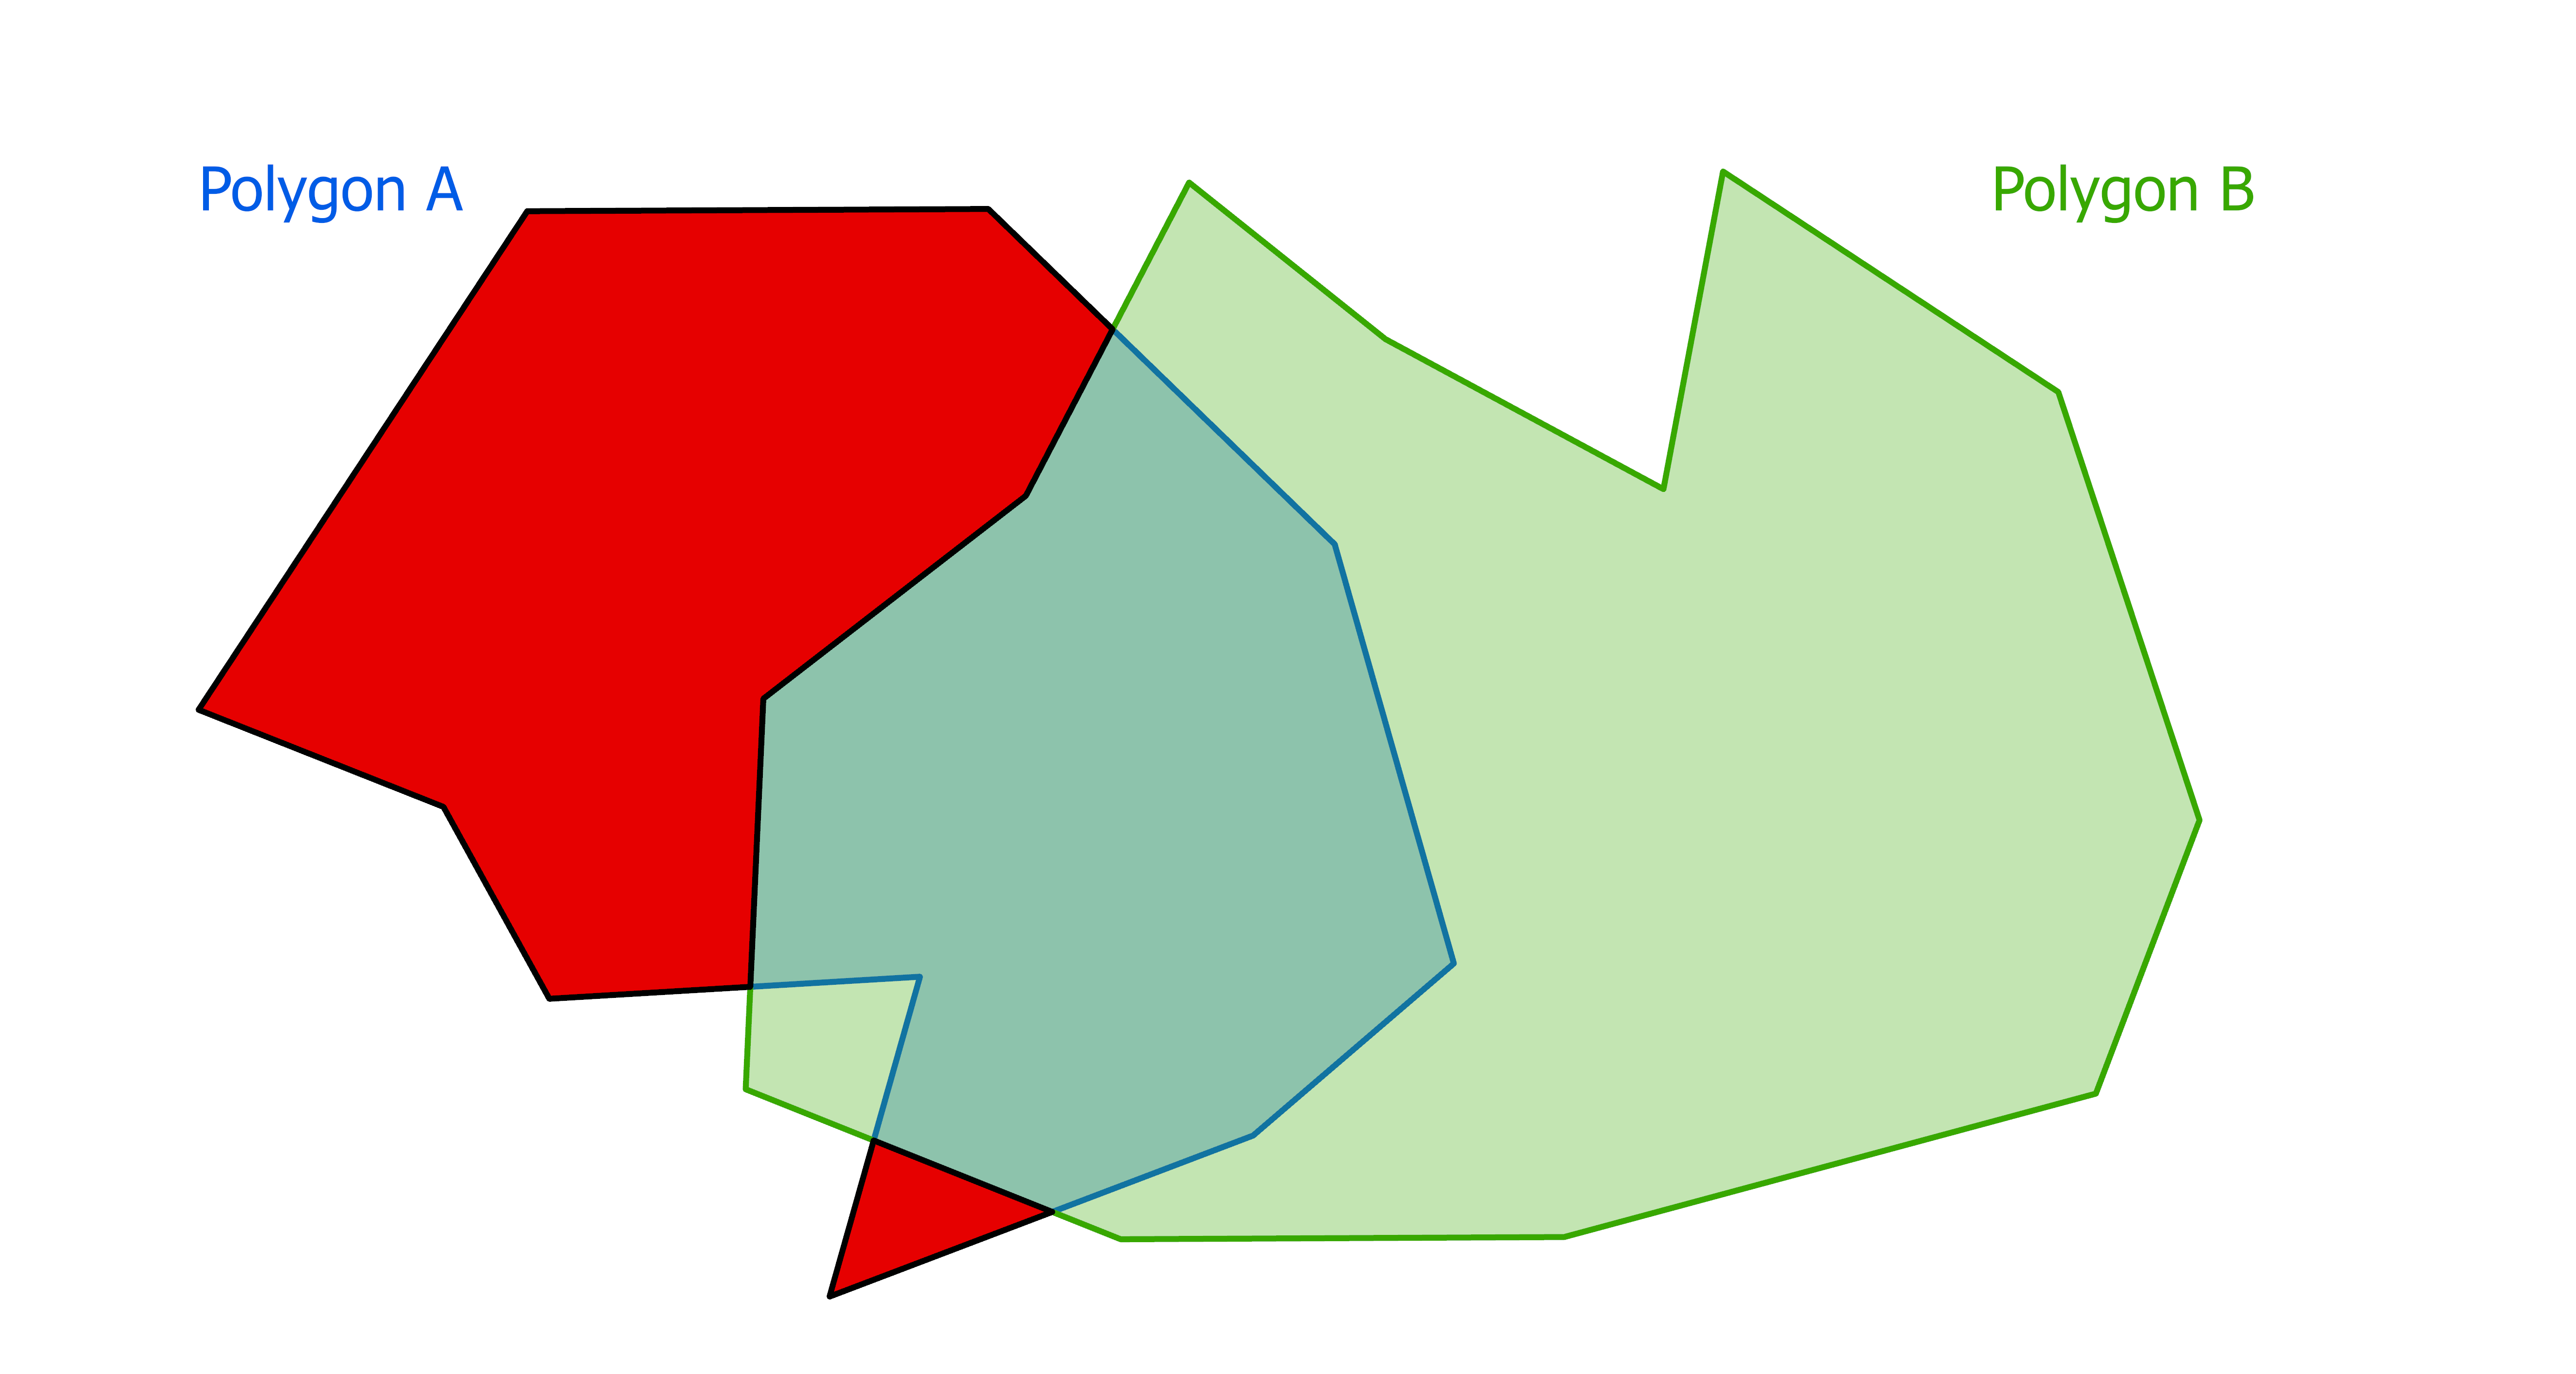
\includegraphics[height=35mm]{images/rozdil_Apng.PNG}\]
\[\textit{\footnotesize{Obr. 4 - Rozdíl polygonů A a B}}\]
\[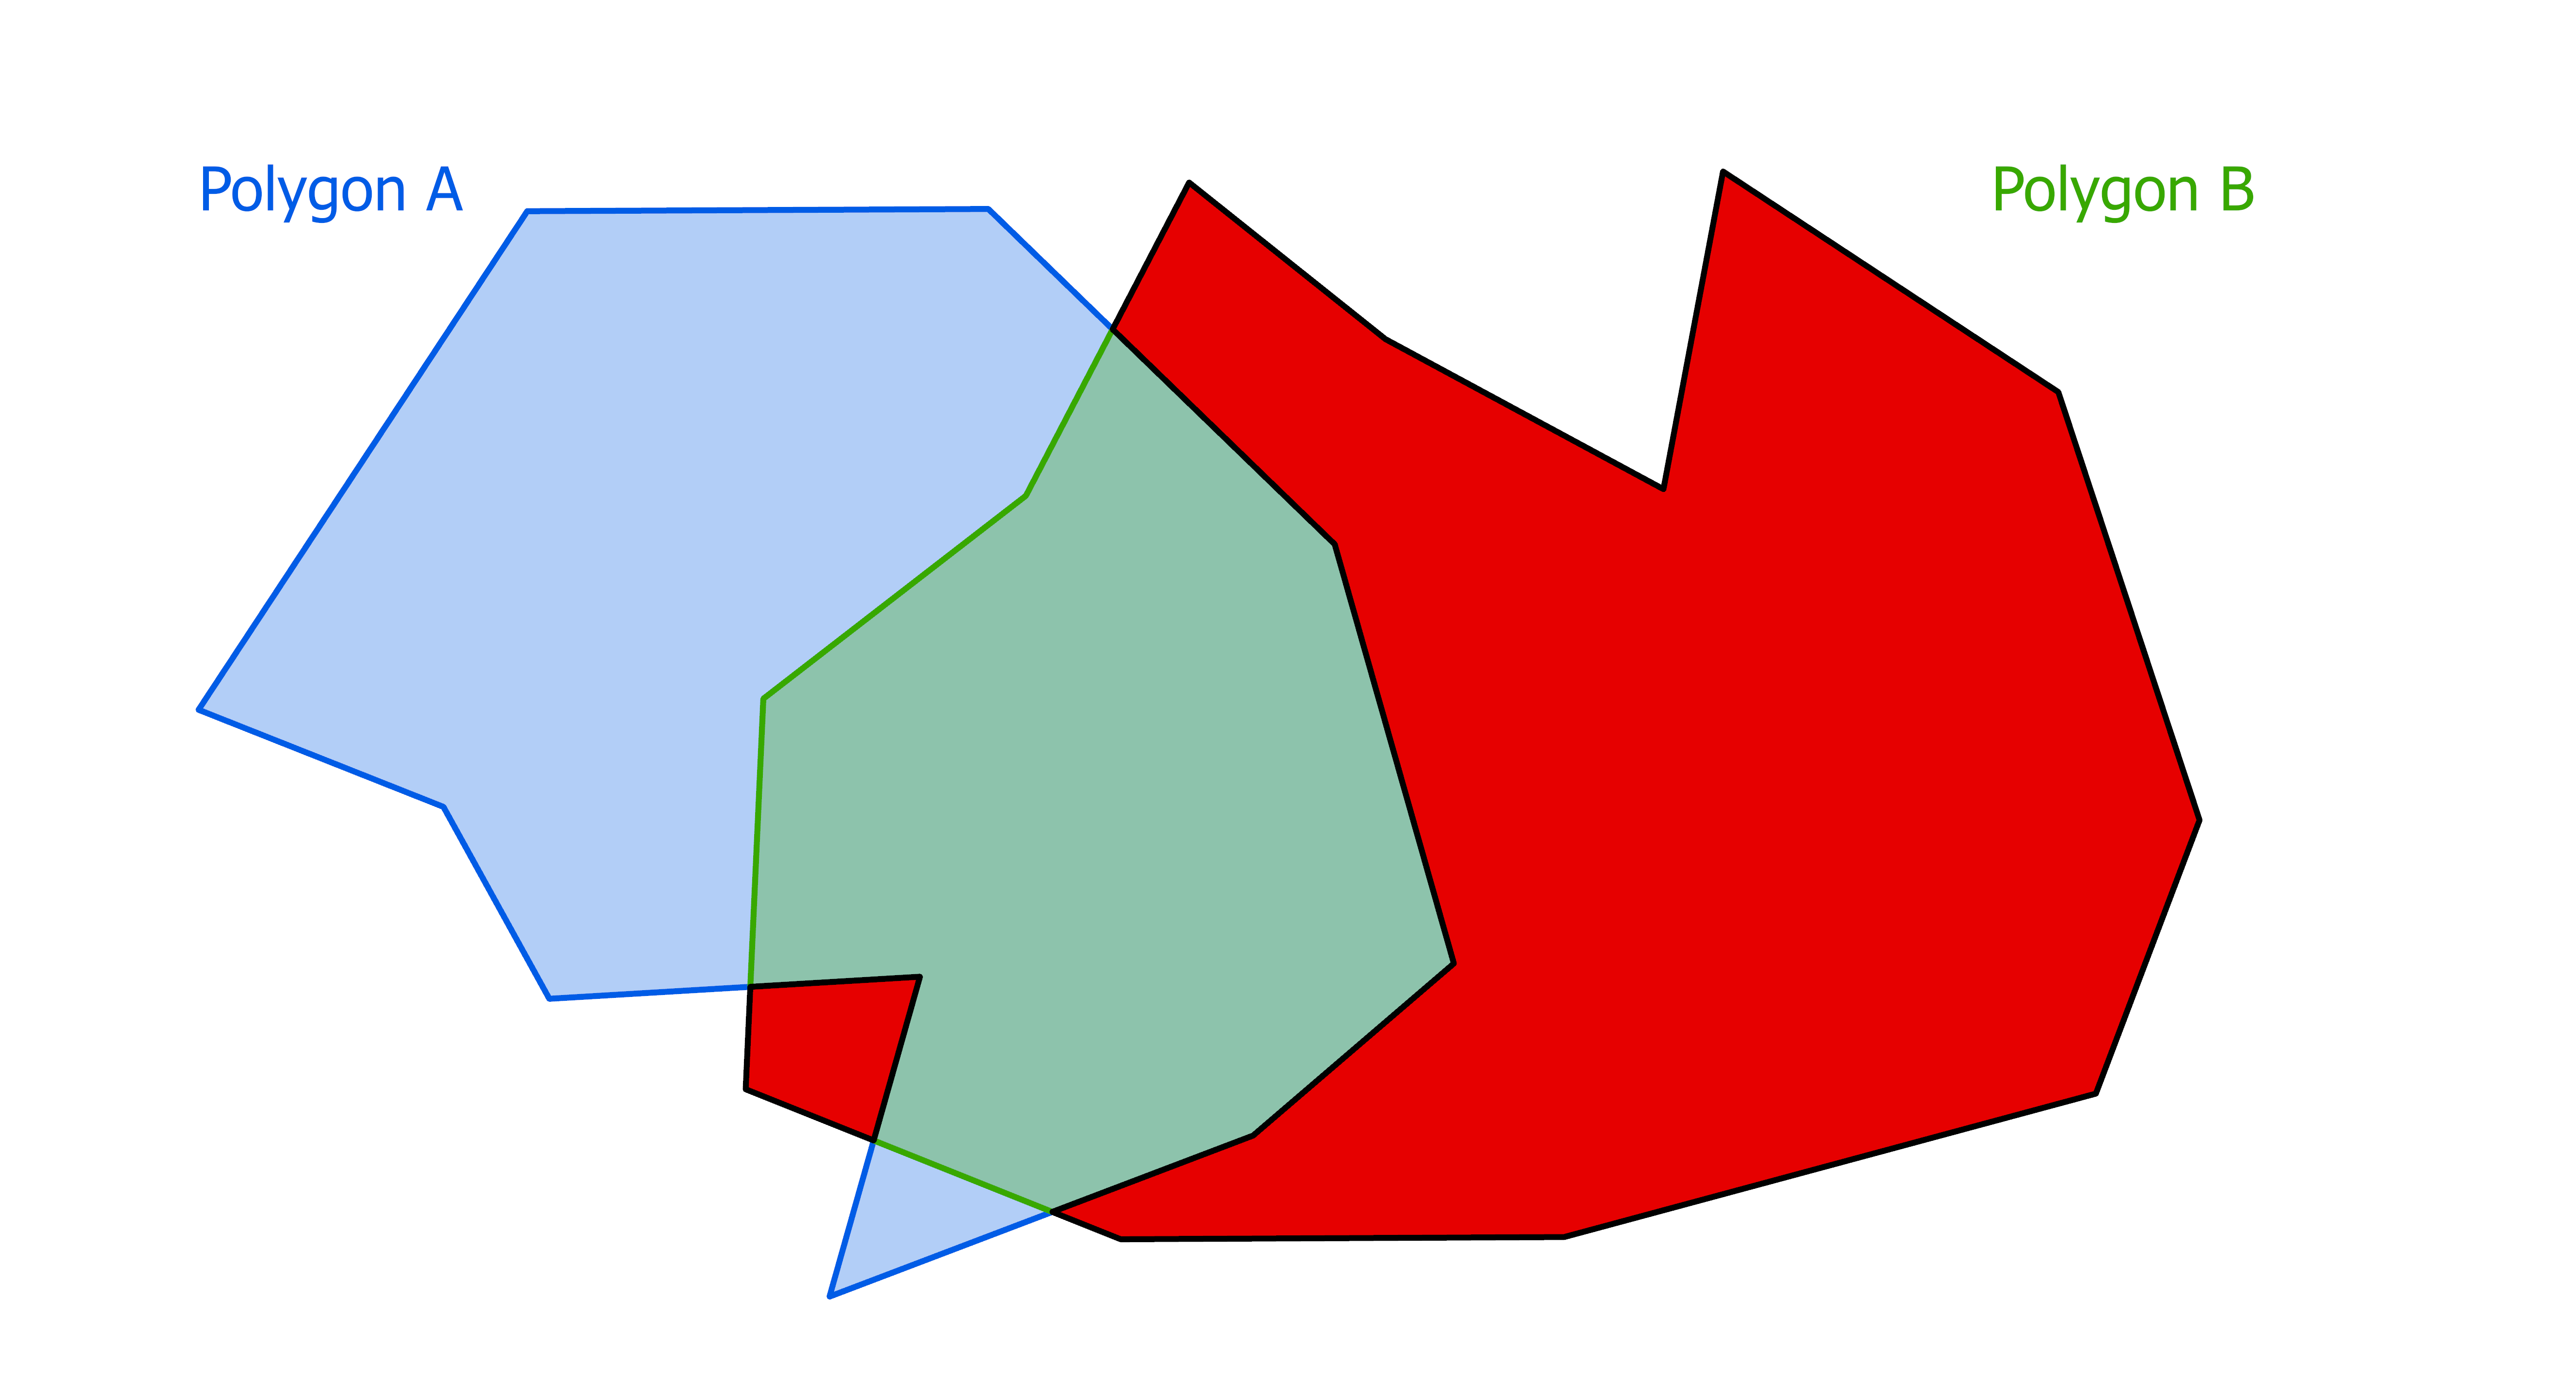
\includegraphics[height=35mm]{images/rozdil_Bpng.PNG}\]
\[\textit{\footnotesize{Obr. 5 - Rozdíl polygonů B a A}}\]
\clearpage
\newpage
\section{\large{Popis algoritmu}}
Základem tohoto algoritmu je \emph{QPointFB}, což je nový datový typ nesoucí informaci o parametrech $\alpha, \beta$. Tyto parametry charakterizují polohu průsečíků dvou hran uvnitř těchto dvou hran. Datový typ \emph{QPointFB} navíc obsahuje informaci o poloze bodu vůči polygonu. Do algoritmu vstupují polygony $A =\{p_{i}\}_{i=1}^n$ a~$B =\{q_{j}\}_{j=1}^m$, jejichž první a poslední bod je totožný a jehož orientace je proti směru hodinových ručiček.
\subsection{\small{Výpočet průsečíků}}
Na začátku je potřeba vypočítat průsečík $b_{ij}$ hran $A, B$, pokud existuje. Nejprve je potřeba zjistit vzájemnou pozici hran, jelikož chceme pouze ty, které se protínají. Vypočítají se směrové vektory $\vec{u}, \vec{v}, \vec{w}$ pro~hrany $e_{i} = (p_{i}, p_{i+1}),~e'_{j} = (q_{j}, q_{j+1})$, kde určíme $p_{i} = [x_{i}, y_{i}],~p_{i+1} = [x_{i+1}, y_{i+1}],~q_{j} = [x_{j}, y_{j}],~q_{j+1} = [x_{j+1}, y_{j+1}]$:\\
\[\vec{u} = (x_{i+1} - x_{i}, y_{i+1} - y_{i}),\]
\[\vec{v} = (x_{j+1} - x_{j}, y_{j+1} - y_{j}),\]
\[\vec{w} = (x_{i} - x_{j}, y_{i} - y_{j}).\]
\vspace{0cm}\\
Poté dopočítáme determinanty $k_{1}, k_{2}, k_{3}$\\
\[k_{1} = v_{x} \cdot w_{y} - v_{y} \cdot w_{x},\]
\[k_{2} = u_{x} \cdot w_{y} - u_{y} \cdot w_{x},\]
\[k_{3} = v_{y} \cdot u_{x} - v_{x} \cdot u_{y},\]
\vspace{0cm}\\
z nichž vypočítáme parametry $\aplha, \beta$\\
\[\alpha = \frac{k_{1}}{k_{3}},\]
\[\beta = \frac{k_{2}}{k_{3}}.\]
\vspace{0cm}\\
V případě $k_{1} = 0, k_{2} = 0, k_{3} = 0$ jsou hrany $e_{i}, e'_{j}$ kolineární.\\
V případě $k_{1} = 0, k_{2} = 0$ jsou hrany $e_{i}, e'_{j}$ rovnoběžné.\\
V předchozích případech průsečík neexistuje. V případě, kdy průsečík existuje jako $0 \leq \alpha \leq 1$ a $0 \leq \beta \leq 1$, je potřeba přepočítat jeho souřadnice X, Y\\
\[X = p_{1x} + \alpha u_{x},\]
\[Y = p_{1y} + \alpha u_{y}.\]
\vspace{0cm}\\
V každém dalším případě jsou hrany $e_{i}, e'_{j}$ mimoběžné.
\subsection{\small{Vkládání průsečíků do polygonů}}
Může nastat situace, kdy hrana $e$ polygonu $A$ protne hranu $e'$ polygonu $B$ více než jednou (a naopak). Kvůli tomu je nutné testovat hranu $A$ vůči všem hranám polygonu $B$. Pokud existuje průsečík $b_{ij}$, bude přidán do polygonu $B$ na pozici $i + 1$. Aby byl průsečík přidaný i do polygonu $A$, musí být průsečík přidaný do slovníku $D$. Slovník $D$ je přidaný do polygonu $A$ po nalezení všech průsečíků.
\subsection{\small{Ohodnocení vrcholů polygonů}}
Dále bude probíhat ohodnocení vrcholů $A, B$, které závisí na určení polohy polygonu vůči druhému polygonu. O poloze $e_{i} = (p_{i}, p_{i+1})$ k $B$ rozhoduje poloha vnitřního bodu, která se vypočítá jako\\
\[\overline{p_{i}} = 0,5(p_{i} + p_{i + 1}).\]
\vspace{0cm}\\
Analogicky poloha $e'_{j} = (q_{j}, q_{j+1})$ k $A$ se vypočítá jako\\
\[\overline{q_{i}} = 0,5(q_{j} + q_{j + 1}).\]
\vspace{0cm}\\
Každému $\overline{p_{i}} \in A$ určíme polohu vzhledem k $B$ a každému $\overline{q_{i}} \in B$ určíme polohu vzhledem k $A$. Z ohodnocovací funkce $g$ víme, že \begin{equation}
    g(e_{i}, B) = g(\overline{p_{i}}, B) = \begin{cases}
             vně,~$\overline{p_{i}} \notin B$,\\
             na~hranici~A/B,~$\overline{p_{i}} \in \partial B$,\\
             uvnitř,~$\overline{p_{i}} \in B$.\\
    \end{cases}
\end{equation}
\begin{equation}
    g(e'_{j}, A) = g(\overline{q_{j}}, A) = \begin{cases}
             vně,~$\overline{q_{j}} \notin A$,\\
             na~hranici~A/B,~$\overline{q_{j}} \in \partial A$,\\
             uvnitř,~$\overline{q_{j}} \in A$.\\
    \end{cases}
\end{equation}
\subsection{\small{Výběr hran podle pozice}}
Následuje výběr hrany podle pozice. Jsou vybrány hrany z obou polygonů, které měly k druhému polygonu konkrétní pozici (určené výše). Bude se procházet přes všechny vrcholy polygonu. Pokud se rovná pozice bodu se zadanou pozicí, tak se z tohoto bodu a jeho následujícího bodu vytvoří hrana. Z polygonu $A$, respektive $B$,~jsou v případě průniku vybrané ty hrany uvnitř polygonu $A$, respektive $B$. V případě sjednocení jsou z polygonu $A$, respektive $B$, vybrány ty hrany mimo polygon $A$, respektive $B$. V případě rozdílu $B-A$ jsou z polygonu $B$ vybrány hrany mimo polygon $A$, které jsou zároveň uvnitř polygonu $B$. Opačně to platí v případě rozdílu $A-B$.
\clearpage
\newpage
\section{\large{Dokumentace}}
Program je rozdělen do 10 modulů. Modul \texttt{mainform.py} je převážně vygenerován pomocí softwaru QT Creator a slouží k vytvoření uživatelského rozhraní a k volání jednotlivých funkcí pomocí tlačítek v UI. (Obr. 1) Modul \texttt{algorithm.py} obsahuje algoritmy pro množinové operace s polygony. Modul \texttt{draw.py} slouží především pro propojení předešlých dvou modulů a k zajištění vizualizace vstupu a výstupu. Modul \texttt{input.py} zajišťuje nahrání vstupních dat v požadovaném formátu. Modul \texttt{QPointFB.py} upravuje třídu \texttt{QPointF} tak, aby body obsahovaly informaci o poloze vůči druhému polygonu a informace o poloze na hranách polygonů (od počátku hrany). Modul \texttt{edge.py} definuje třídu \texttt{Edge}, která definuje datový typ hrany. Hrana v sobě nese informaci o počátečním a koncovém bodě. Moduly \texttt{booleanoperations.py}, \texttt{lineandlineposition.py}, \texttt{pointandpolygobposition.py} a \texttt{pointlineposition.py} definují třídy odvozené z třídy \texttt{Enum}. Mají za úkol přiřadit hodnotám jejich slovní název.
\[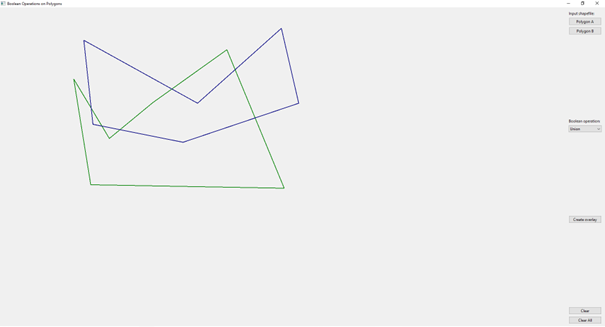
\includegraphics[height=90mm]{images/app.PNG}\]
\[\textit{\footnotesize{Obr. 1 - Náhled uživatelského rozhraní}}\]
\subsection{\small{Modul mainform.py}}
Tento modul obsahuje třídu \texttt{Ui\_Mainform}, která je vytvořena automaticky pomocí QT Creatoru. Tato třída byla posléze doplněna o metody, které se spustí při interakci s uživatelským rozhraním. Jedná se o metody \emph{inputA}, \emph{inputB}, \emph{clickCreateOverlay}, \emph{clickclear} a \emph{clickclearALL}. Metody \emph{inputA} a \emph{inputB} slouží k vyvolání funkce \emph{loadFile} z modulu \texttt{input.py}, čímž nahrají vstupní polygony. Metoda \emph{clickCreateOverlay} provede zvolenou množinovou operaci se vstupními polygony. Metoda \emph{clickclear} slouží k odstranění výsledku a metoda \emph{clickclearALL} pro odstranění všeho.
\subsection{\small{Modul input.py}}
Tento modul obsahuje metodu \emph{loadfile}. V této metodě je nejprve načtena cesta ke vstupním datům. Když není zvolena žádná cesta, metoda se ukončí. Dále je načten vstupní textový dokument, z něhož jsou získány vrcholy polygonu.
\subsection{\small{Modul draw.py}}
Tento modul obsahuje třídu \texttt{Draw}, kterou dědí od třídy \texttt{QWidget} z knihovny PyQt6. Hlavní funkcí tohoto modulu je vykreslit vstupní polygony a následně výsledky množinových operací. Polygony $A$ a $B$ jsou uloženy v proměnných \emph{polA} a \emph{polB} ve formátu listů obsahující jednotlivé vrcholy, které jsou ve formátu \emph{QPointFB}. Výsledek množinové operace je v proměnné \emph{res}, která je opět list, který obsahuje hrany ve formátu \emph{edge}.
\subsection{\small{Modul algorithm.py}}
Zde se nacházejí jednotlivé funkce pro množinové operace s polygony. V modulu se nachází jediná třída \emph{Algorithms}, která obsahuje níže uvedené metody.\\
Metoda \emph{getPointAndLinePosition} má na vstupu 3 body \emph{QPointFB}, kde 2 body definují přímku a zbylý bod definuje analyzovaný bod. Tato metoda zjistí, ve které polorovině se analyzovaný bod nachází. Výsledek je vracen ve formátu výčtové třídy definované v modulu \texttt{pointlineposition.py}. Hodnoty jsou definovány takto:\begin{itemize}
    \item Left\_HP (1) pro bod v levé polorovině,
    \item Right\_HP (-1) pro bod v pravé polorovině,
    \item On\_Line (0) pro kolineární bod.
\end{itemize}
Metoda \emph{get2LinesAngle} má na vstupu 4 body \epmh{QPointFB}, které definují 2 přímky, u nichž je zjišťován úhel, který spolu svírají.\\
Hlavní metoda této třídy - \emph{getPositionPointAndPolygon} - zjišťuje vzájemnou polohu daného bodu ve formátu \emph{QPointFB} a polygonu definovaného jako list \emph{QPointFB}. Výstup je ve formátu výčtové třídy definované v modulu \texttt{pointandpolygonposition.py}. Vrácené hodnoty jsou: \begin{itemize}
    \item Inside (1) pro bod uvnitř,
    \item Outside (0) pro bod vně,
    \item Boundary (-1) pro bod na hraně polygonu.
\end{itemize}
Tato metoda je založena na algoritmu \emph{Winding Number}.\\
Metoda \emph{get2LinesIntersection} vrací vzájemnou polohu dvou vstupních úseček, které jsou definovány čtyřmi body \emph{QPointFB}. Výsledek je opět ve formátu výčtové třídy definované v modulu \emph{lineandlineposition.py}, a to jako: \begin{itemize}
    \item Parallel (1) pro rovnoběžné úsečky,
    \item Skew (2) pro mimoběžné úsečky,
    \item Colinear (3) pro úsečky kolineární,
    \item Intersect (4) pro úsečky s jedním průsečíkem.
\end{itemize}
Metoda \emph{updateVertices} přidá body do hran dvou vstupních polygonů v místě, kde se jejich hrany vzájemně kříží. Vstupní polygony jsou list \emph{QPointFB}. Výstup tato funkce nemá, pouze aktualizuje vstupní polygony.\\
Metoda \emph{setEdgePosition} přiřadí jednotlivým hranám vstupního polygonu polohy vůči polygonu druhému. Vstupem jsou tedy 2 polygony definovány jako list \emph{QPointFB}. Polohy jsou vztaženy ke středu hrany a jsou ukládány do atributu \emph{position} prvního bodu definující hranu. Poloha je získána pomocí metody \emph{getPositionPointAndPolygon}.\\
Metoda \emph{getEdges} vybere hrany vstupního polygonu, které mají pozici vůči druhému polygonu stejnou, jako je vstupní parametr metody. Na vstupu jsou tedy tři proměnné, polygon list \emph{QPointFB}, žádaná pozice hrany určená pomocí výčtové třídy \texttt{PointAndPolygonPosition} a hrany, definované jako list \emph{edges}. Výstupem je aktualizovaný list hran.\\
Metoda \emph{createOverlay} provede zvolenou množinovou operaci polygonů. Na vstupu jsou 2 polygony jako list \emph{QPointFB} a množinová operace definována výčtovou třídou \emph{BooleanOperation} z modulu \texttt{booleanoperation.py}. Výstupem je list hran, které splňují danou množinovou operaci.
\subsection{\small{Modul Uživatelské datové typy}}
V modulech \texttt{edge.py} a \texttt{qpointfb} jsou definovány uživatelské datové typy. Uživatelský datový typ \emph{QPointFB} je odvozen od třídy \texttt{QPointF}. Stejně jako \emph{QPointF} nese informaci o poloze bodu v osách x a y. Následně ještě přidává hodnotu $\alpha$ a $\beta$, které určují polohu průsečíku dvou hran. Tyto atributy nabývají hodnoty z intervalu (0, 1) pro body, které jsou průsečíkem hran. Poté je ještě přidán atribut \emph{position}, který reflektuje pozici středu hrany vůči druhému polygonu. Datový typ \emph{Edge} definuje hrany jako začáteční a koncový bod typu \emph{QPointFB}.\\
Pseudokódy konkrétních metod jsou uvedeny níže.
%-------------------------------------get2LinesIntersection--------------------------------------%
\vspace{0,2cm}\\
\indent\textit{\textbf{get2LinesIntersection:}}\\
\indent\textit{Vypočti směrové vektory $u(p_{1}p_{2}), v(p_{3}p_{4}), w(p_{1}p_{3})$, kde $p_{i}$ jsou body definující 2 úsečky}\\
\indent\textit{Vypočti koeficienty $k_{1}, k_{2}$ a $k_{3}$}\\
\indent\textit{\textbf{Když} $k_{3} = 0$:}\\
\indent\indent\textit{Vrať úsečky jsou kolineární, bod průsečíku je None}\\
\indent\textit{Vypočti parametry $\alpha$ a $\beta$}\\
\indent\textit{\textbf{Když} $k_{1} a k_{2} = 0$:}\\
\indent\indent\textit{Vrať úsečky jsou paralelní, bod průsečíku None}\\
\indent\textit{\textbf{Když} $0 \leq \alpha \leq 1$ a $0 \leq \beta \leq 1$:}\\
\indent\indent\textit{Získej hodnotu průsečíku jako:}\\
\indent\indent\textit{$X = p_{1x} + \alpha u_{x}, Y = p_{1y} + \alpha u_{y}$}\\
\indent\textit{Definuj průsečík QPointFB $q(x, y, \alpha, \beta)$}\\
\indent\textit{Vrať úsečky mající průsečík q}\\
%-------------------------------------updateVertices--------------------------------------%
\vspace{6,5cm}\\
\indent\textit{\textbf{updateVertices:}}\\
\indent\textit{Inicializuj index i = 0}\\
\indent\textit{\textbf{Dokud} i $<$ počet vrcholů a polygonu A:}\\
\indent\indent\textit{Inicializuj slovník D}\\
\indent\indent\textit{inicializuj index j = 0}\\
\indent\indent\textit{\textbf{Dokud} j < počet vrcholů b polygonu B:}\\
\indent\indent\indent\textit{Získej průsečík dvou hran $h_{1}(a_{i},a_{i+1}),h_{2}(b_{j},b_{j+1})$}\\
\indent\indent\textit{\textbf{Když} mají právě jeden průsečík:}\\
\indent\indent\indent\textit{Získej polohu průsečíku I na obou aktuálních hranách jako $\alpha$ a $\beta$}\\
\indent\indent\indent\textit{Přidej průsečík do D, kde key je hodnota, $\alpha$ item je I}\\
\indent\indent\indent\textit{Inkrementuj j = j + 1}\\
\indent\indent\indent\textit{Přidej průsečík do polygonu B na pozici j}\\
\indent\indent\textit{Inkrementuj j = j + 1}\\
\indent\textit{\textbf{Dokud} i < počet vrcholů a polygonu A:}\\
\indent\textit{\textbf{Když} existuje nějaký průsečík v D:}\\
\indent\indent\textit{\textbf{Pro} všechny záznamy v seřazených podle hodnoty klíče k ve slovníku:}\\
\indent\indent\indent\textit{Inkrementuj i = i + 1}\\
\indent\indent\indent\textit{Vlož do vrchol v do polygony A na pozici i}\\
\indent\indent\textit{Inkrementuj i = i + 1}\\
\subsection{\small{Vstup}}
Vstupní polygony jsou nahrány do uživatelského rozhraní pomocí tlačítek \emph{Polygon A} a \emph{Polygon B}. Každé tlačítko slouží pro nahrání jednoho polygonu. Data jsou v textovém dokumentu tak, že jsou zde zapsány na každém řádku souřadnice jednotlivých vertexů polygonu. Souřadnice x a y jsou odděleny mezerou. Souřadnice jsou vztaženy k souřadnicím zobrazovacího okna (tzn. od 0, 0 až po maximální rozměry obrazovky).
\subsection{\small{Výstup}}
Výstup je zajištěn graficky tak, že jsou zvýrazněny hrany, které splňují zvolenou množinovou operaci.~(Obr.~2)
\[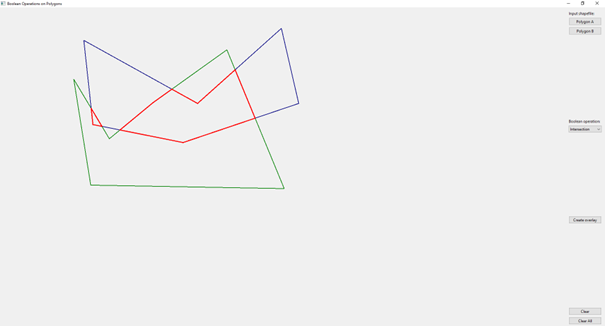
\includegraphics[height=90mm]{images/app_4.PNG}\]
\[\textit{\footnotesize{Obr. 2 - Výstup operace Intersection (červeně)}}\]
\clearpage
\newpage
\section{\large{Závěr}}
Program vyhodnotí zvolenou množinovou operaci dvou vstupních polygonů. U programu by mohl být vylepšen vstupní formát tak, aby mohly být jednotlivé polygony nahrávány například ve formátu \emph{.shp} či aby byly například v JTSK (pro lepší aplikaci na reálná data). 
\clearpage
\newpage
\section{\large{Zdroje}}
MORAVEC, L. (2008) - Webová aplikace pro výuku matematické logiky na střední škole. Diplomová práce. Univerzita Karlova, Matematicko-fyzikální fakulta, Praha, 168 s.\\
Přednášky z předmětu \emph{Algoritmy počítačové kartografie}
\end{document}
